\chapter{GoLightly} \label{ch:golightly}

GoLightly is the GPU-based FDTD simulator application that is the focus and product of this thesis. Written using a combination of C++, CUDA and OpenGL, it provides a lightweight yet complete FDTD solution.

\section{Goals}

GoLightly is intended to address deficiencies common to CPU-based solutions. In particular, it is designed to be fast, friendly and portable.


\begin{itemize}
	\item Fast. An iterative design process requires rapid feedback from the simulator. Long simulation times necessitated by existing solutions inhibit this process.
	\item Friendly. Definition of models and other simulation parameters should not require expertise in software development or quasi-proprietary scripting languages. 
	\item Portable. Ideally, the simulator should run on a high-end consumer grade laptop and support the most common desktop operating systems (Microsoft Windows and Apple OS X).  
\end{itemize}

To meet those goals, GoLightly takes advantage of the oft-underutilized programmable GPU available in common desktop and laptop computers, resulting in a dramatic speedup. Rather than relying on a proprietary model definition language or obscure, limited scripting system, we use industry-standard image and geometry file formats so that models may be defined using robust, familiar, readily-available tools. By building the software specifically for Microsoft Windows, we ensure that it is compatible with the most common desktop operating system. 

\section{Architecture}

GoLightly comprises three primary application blocks:

\begin{itemize}
	\item Model Processor \ref{sec:modelProcessor}
	\item Simulator \ref{sec:simulator}
	\item Visualizer \ref{sec:visualizer}
\end{itemize}


FLOWCHART HERE?

\subsection{Model Processor}\label{sec:modelProcessor}

The model processor (MP) is responsible for initialization of the simulator. When launching the simulator, a domain size and image file, containing a coded image of the desired dielectric, as well as a max $\epsilon$ are specified.

\begin{table}[h!]
	\centering
	\caption{Model processor inputs}
	\label{tab:modelProcessorInputs}
	\begin{tabular}{l | l | l | l}
		Symbol	& Data Type & Meaning & Typical value				\\
		\hline														\\
		Width	& int 		& Domain size in X & 1024				\\
		Height	& int 		& Domain size in Y & 1024				\\
		Media	& float 	& $\epsilon_{max}$ & 9						\\
		Model	& string	& Model definition stored as a bitmap & filename
	\end{tabular}
\end{table}

The MP allocates arrays to hold the dielectric properties for each Yee cell. These arrays are of the same dimensions as the domain, which may be different than the dimensions of the model. 

Once the model image is loaded, the MP iterates through each element in the dielectric array. (See \autoref{listing:modelFromImage})

For each element:

\begin{enumerate}
	\item Determine the normalized texel coordinate that corresponds to the current cell position	
	\item Read the red (R), green (G) and blue (B) color components from the image
	\item If $R > 128$, this texel is part of a source. Add the cell to the list of sources
	\item If $G > 0$, this texel has non-unity dielectric. Set ${C_b}_{i,j} = \epsilon_{max} * \frac{G}{255.0}$
	\item If $B > 0$, this texel is part of a monitor. Add its position to the monitor definition with ID = $B$
\end{enumerate}

\lstinputlisting[language=c++,caption=Generating a model from an image]{model-from-image.cpp}\label{listing:modelFromImage}

Once the dielectric, sources and monitors are derived from the model image, the model processor transfers control to the simulator.

\subsection{Simulator}\label{sec:simulator}

The simulator block implements the FDTD algorithm. Given the dielectric, source and monitor configurations from the model processor, the simulator initializes the GPU, transfers required data from host memory to the GPU, and begins the simulation loop.

In addition to the dielectric and field arrays, the simulator generates a  descriptor (\autoref{listing:fieldDescriptor}) for each field that will be updated. This structure is used by the kernels to assist in handling boundary conditions (PML) and other housekeeping duties. A similar, more compact  descriptor (\autoref{listing:deviceFieldDescriptor}) is generated from the host descriptor and passed to the kernels.

\lstinputlisting[language=c++,caption=Host Field Descriptor structure]{fieldDescriptor.cpp}\label{listing:fieldDescriptor}

\lstinputlisting[language=c++,caption=Device Field Descriptor]{deviceFieldDescriptor.cpp}\label{listing:deviceFieldDescriptor}

For each loop iteration, the simulator launches a CUDA kernel to update all $E$ fields. Once the $E$ update is complete, the simulator launches kernels to update all $H$ fields.

The three kernels required for a $TM_Z$ simulation are detailed below:

\lstinputlisting[language=c++,caption=CUDA kernel for updating $E_Z$]{cu_update_ez.cpp}\label{listing:updateEzCpp}

The majority of each kernel's source performs setup and bounds checking tasks. In each kernel, the FDTD equation implementation can be isolated to one or two lines of code.

For example, the line (from the $E_Z$ update kernel),

\begin{lstlisting}
	Ez->Data[center] = CA * Ez->Data[center] + cb * (dhy - dhx) + cb * (ezxPsi - ezyPsi);
\end{lstlisting}

corresponds to the FDTD $E_Z$ equation. (See \autoref{eq:ezupdate})

\lstinputlisting[language=c++,caption=CUDA kernel for updating $H_X$]{cu_update_hx.cpp}\label{listing:updateHxCpp}

\lstinputlisting[language=c++,caption=CUDA kernel for updating $H_Y$]{cu_update_hy.cpp}\label{listing:updateHyCpp}

Note that all $E$ updates occur simultaneously, as do all H fields. However, given the dependence between the $E$ and $H$ fields, the $E$ field update kernels must complete before the $H$ fields are updated.

The simulator repeats this operation until the application is closed, or the desired number of frames are completed. 

Finally, the completed field arrays are copied to the host from the GPU, and saved to disk in bitmap and CSV format for later analysis. 

\subsection{Visualizer}\label{sec:visualizer}

If enabled \footnote{The visualizer requires some GPU overhead. As such, its use may affect simulator performance.}, the visualizer application block provides interactive display of the simulation. 

When running a simulation, the user may optionally specify a visualizer update frequency, indicating the number of simulation frames that should complete between visualizer updates. This aids in reducing the visualizer's performance impact.

A window and OpenGL context are created using GLFW and the glLoadGen OpenGL extension loader. An OpenGL pixel buffer object (PBO) is allocated to contain a copy\footnote{The PBO may be of different dimensions than the simulation domain. Since the PBO is used only for visualization, it is not necessary for it to contain the full-resolution field.} of the field that the user wishes to see\footnote{The visualizer provides the ability to dynamically select which field(s) should be displayed}. 

The visualizer also creates a screen-aligned quad on which the field texture will be rendered, and allocates an texture object which is then bound to the PBO. 

After the required number of frames have been completed, the visualizer launches a CUDA kernel which samples the selected field and populates the PBO. 

\lstinputlisting[language=c++,caption=CUDA kernel for updating visualizer pixel buffer object]{cu_visualizer_update.cpp}

A completed PBO is bound to a uniform input for a shader (\autoref{listing:basicVertGlsl},\autoref{listing:basicFragGlsl}) which renders the texture to the visualizer window. 

\lstinputlisting[language=c++,caption=Visualizer vertex shader]{basic_vert.glsl}\label{listing:basicVertGlsl}
\lstinputlisting[language=c++,caption=Visualizer fragment shader]{basic_frag.glsl}\label{listing:basicFragGlsl}

This process runs continuously. However, the texture is only updated at the frequency requested by the user when the simulation was launched. 

\begin{figure}[H]
	\centering
	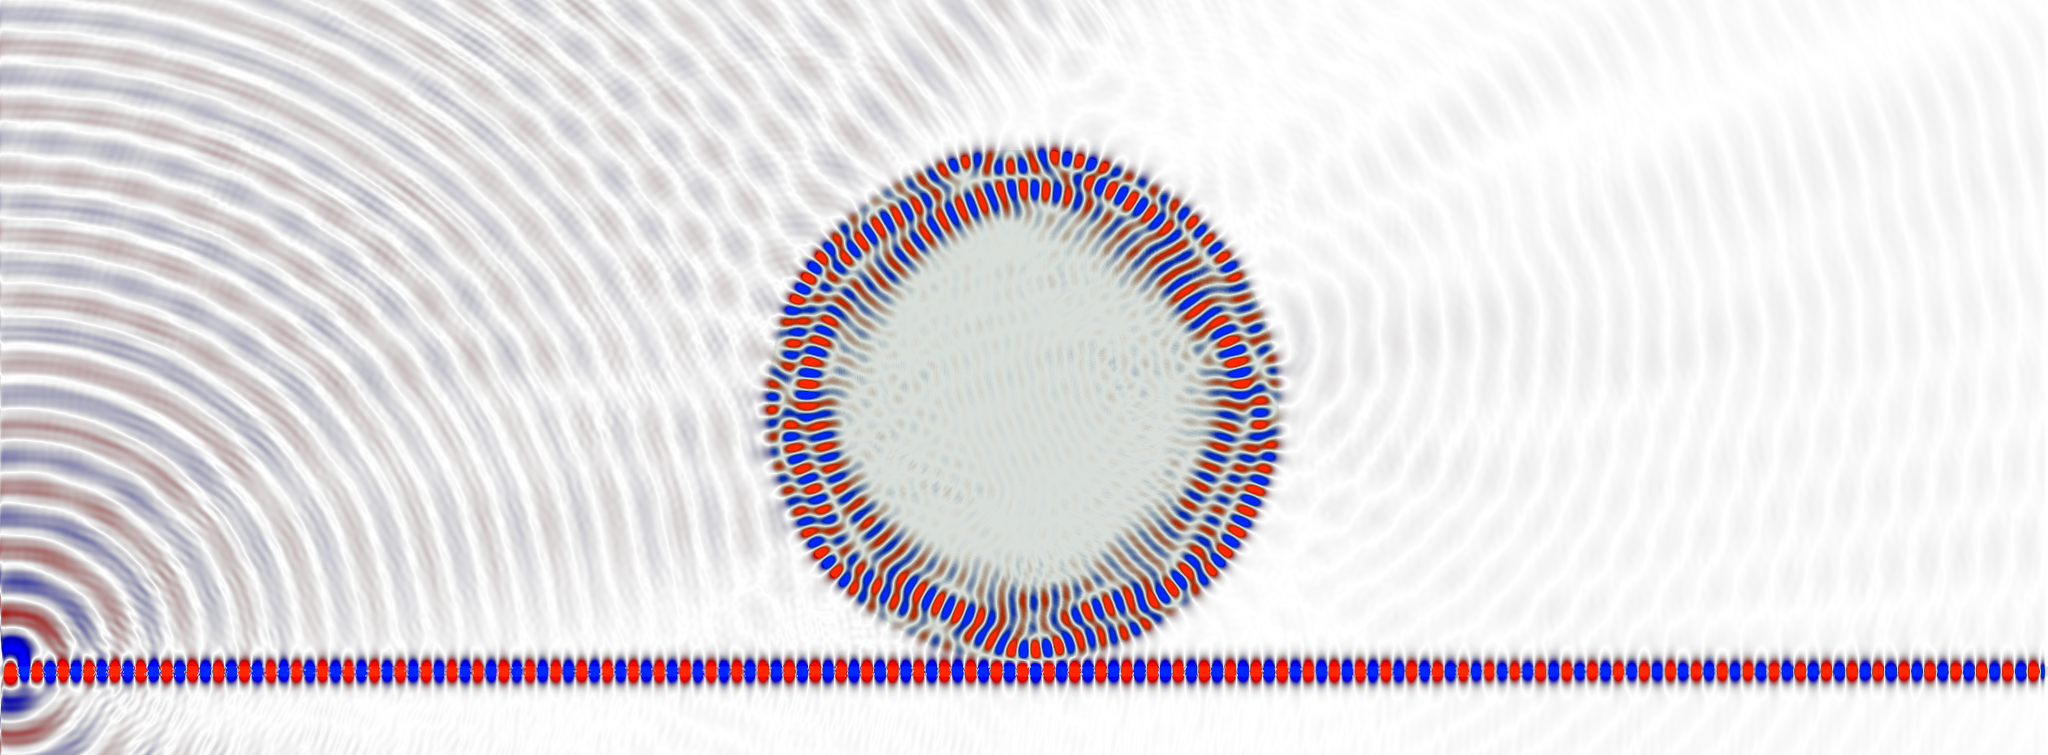
\includegraphics[  width=15cm,
	height=6cm,
	keepaspectratio]{visualizer-wgm.png}
	\caption{2D Whispering Gallery Mode Sensor}
	\label{fig:wgm}
\end{figure}


\section{Modeling approach}

For simplicity, models are defined in any of a number of standard 32-bit color image formats.

In a 32-bit per pixel image, each color has 8-bit red, green, blue and alpha values. As mentioned in the model processor (\autoref{sec:modelProcessor}) section, each component is used to indicate some data about a given point in the simulation domain:

\begin{table}[h!]
	\centering
	\caption{Color component usage}
	\label{tab:modelColorComponentUsage}
	\begin{tabular}{l | l | l}
		Component	& Meaning & Interpretation\\
		\hline															 \\
		Red		& Source 				& scaled frequency of the source \\
		Green	& Dielectric			& $\epsilon_r = green * \frac{\epsilon_{max}}{255.0}$) 	 \\		
		Blue	& Monitor				& ID of the monitor to which this texel belongs \\
		Alpha	& Reserved				& Reserved for future use. \\
	\end{tabular}
\end{table}

Using a tool such as Adobe Photoshop or Microsoft Paint, the user can specify all necessary data - sources, monitors and dielectric - in an intuitive fashion. Alternatively, these bitmaps could be generated by a custom tool which would voxelize a CAD model, assigning color components based on the model's metadata or object properties. 

A significant advantage of this approach over the CSG method used in Meep is that all constructs - sources, monitors and dielectric - can be of any shape that can be drawn in a bitmap. In theory, any 3D voxel-based painting application could be used to build models in higher dimensions. 

\begin{figure}[H]
	\centering
	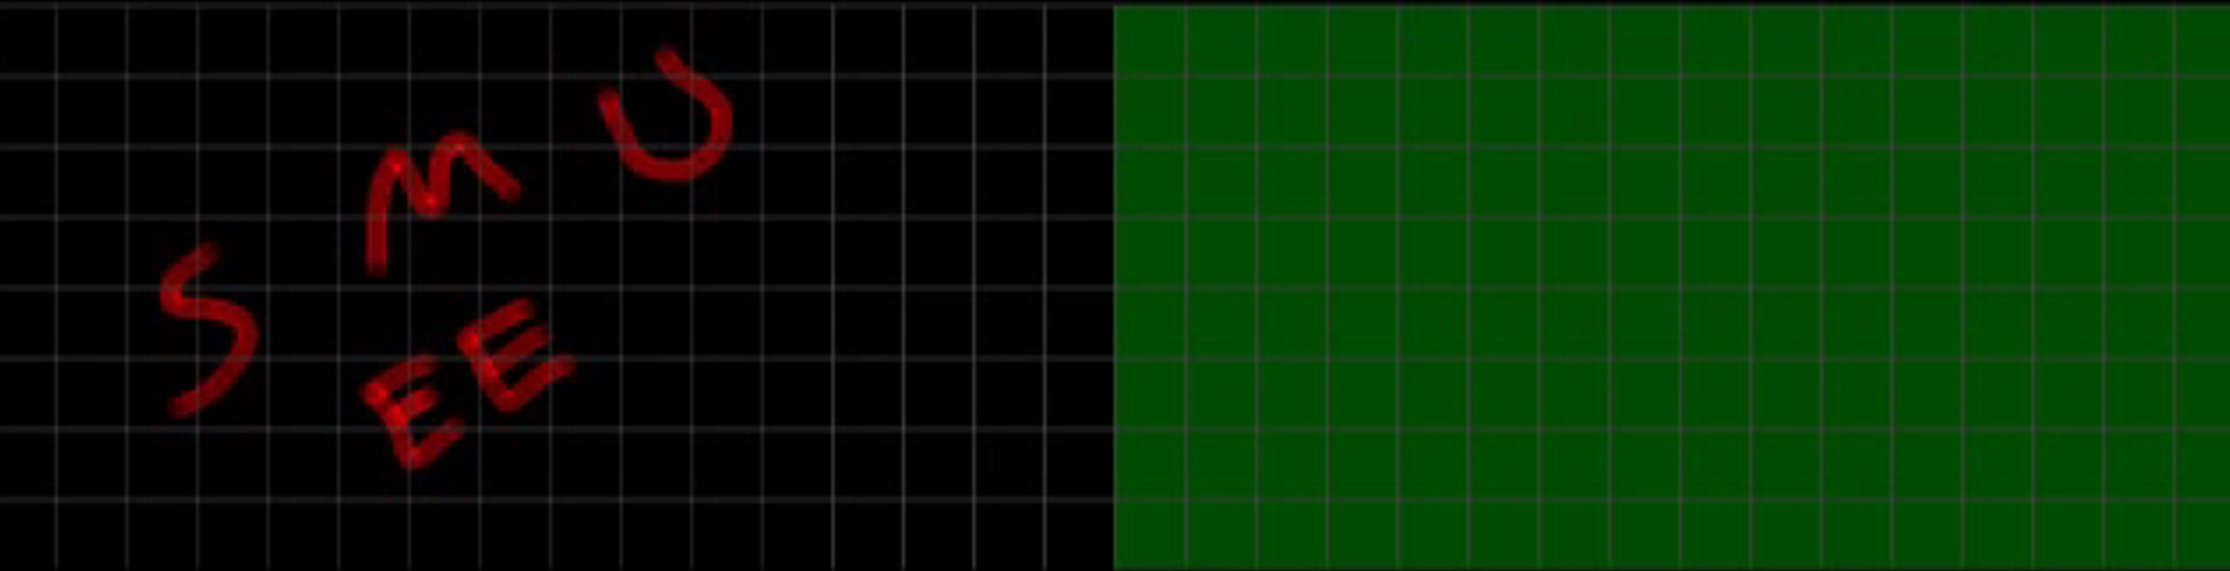
\includegraphics[  width=15cm,
	height=6cm,
	keepaspectratio]{arbitrary-source-shape.png}
	\caption{Arbitrarily-shaped source (Red pixels)}
	\label{fig:arbitrarySource}
\end{figure}

\begin{figure}[H]
	\centering
	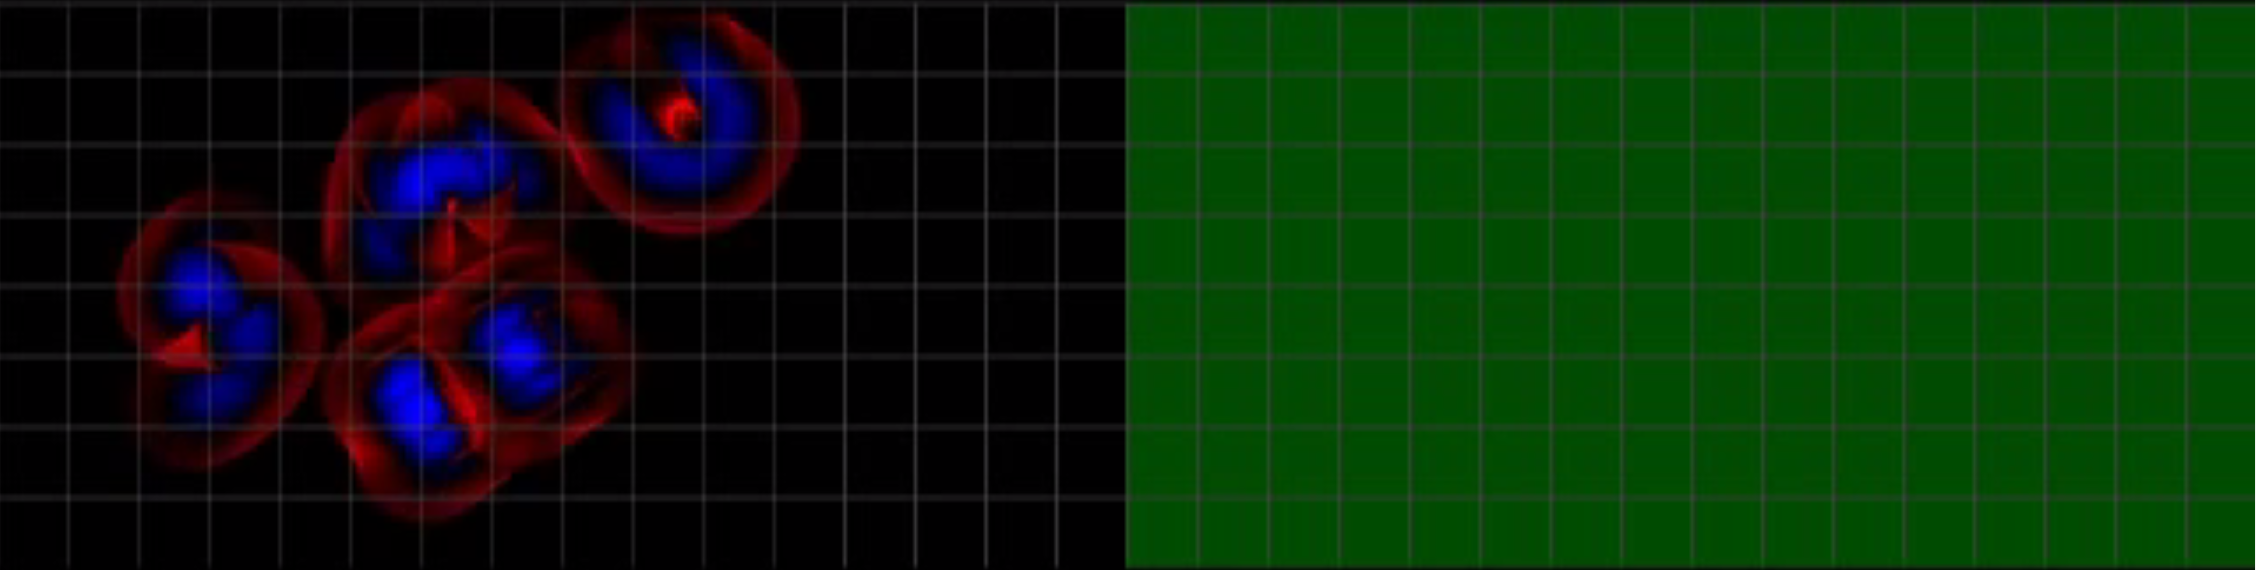
\includegraphics[  width=15cm,
	height=6cm,
	keepaspectratio]{arbitrary-source-shape2.png}
	\caption{Arbitrarily-shaped source after 20 frames}
	\label{fig:arbitrarySource2}
\end{figure}

\begin{figure}[H]
	\centering
	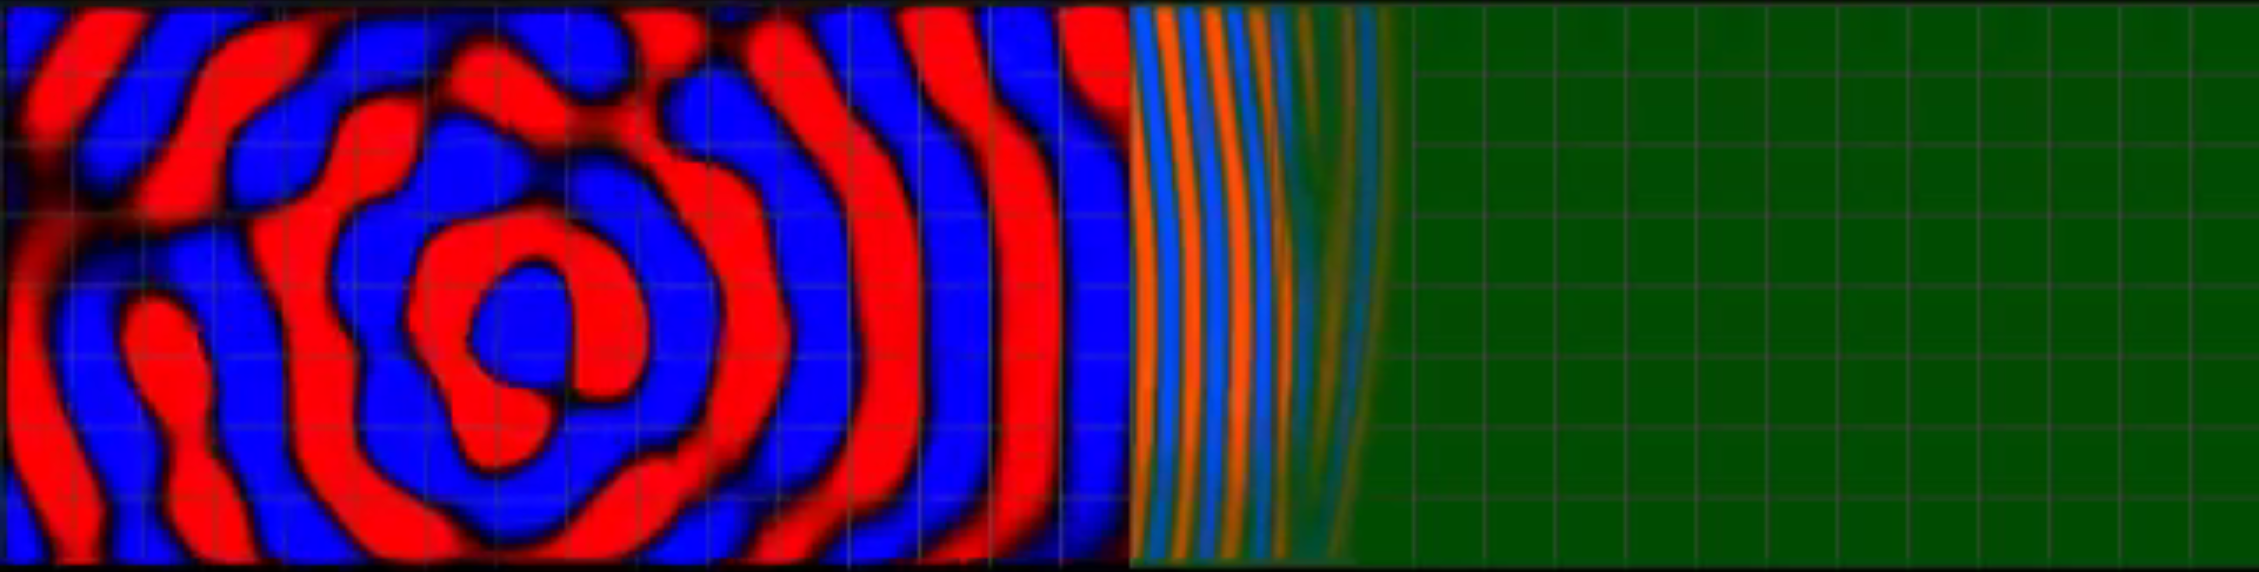
\includegraphics[  width=15cm,
	height=6cm,
	keepaspectratio]{arbitrary-source-shape3.png}
	\caption{Arbitrarily-shaped source after 100 frames}
	\label{fig:arbitrarySource3}
\end{figure}




\section{Testing methodology}
\subsection{Test Model}
\subsection{Analytical Result}
\subsection{Numerical Result}
\subsection{Comparison}
\section{Additional Examples}
\subsection{Coupler}
\subsection{Splitter}

